\vspace{-0.5em}
\section{Experiments}
\label{sec:experiments}



We present results obtained by our method and compare them to the latest state-of-the-art (SOTA) long video understanding models such as VideoBERT~\cite{sun2019videobert}, ViS4mer~\cite{islam2022long}, Turbo~\cite{Han22b} and VideoMamba~\cite{li2024videomamba}. In particular, we show that LV-MAE outperforms previous SOTA methods on downstream tasks from diverse domains such as movies, activity prediction, and procedural tasks. Additionally, we perform thorough ablation studies to assess the effectiveness of various design choices in our approach. We provide implementation details in App.~\ref{app:implementation_details}.



\subsection{Benchmarks}
\paragraph{Long-Video Understanding (LVU).} A challenging suite of tasks aimed at testing models' capabilities in understanding extended movie clips~\cite{wu2021towards}.
The benchmark consists of nine diverse tasks divided into three main categories: content understanding, metadata prediction, and user engagement prediction.
The \emph{content understanding} tasks involve predicting attributes like ``relationship'', ``speaking style'', and ``scene/place''. \emph{Metadata prediction} tasks focus on identifying movie-related attributes such as ``director'', ``genre'', ``writer'', and ``release year''.
Lastly, the \emph{user engagement} tasks measure how well the model can predict YouTube-based metrics such as the ``like ratio'' and ``popularity''. 
The LVU benchmark is built from the MovieClip dataset that is comprising approximately 30,000 videos sourced from around 3,000 movies. 
Each video spans one to three minutes, reflecting real-world movie scenes that require both short-term and long-term temporal reasoning.
\vspace{-1.5em}
\paragraph{Breakfast.} Video classification of cooking activities.
The dataset~\cite{kuehne2014language} consists of 1,712 videos, covering 10 complex cooking activities and totaling 77 hours of footage.
\vspace{-1.5em}
\paragraph{COmprehensive INstruction video analysis (COIN).}
Video classification of procedural tasks depicted in videos.
The COIN dataset~\cite{tang2019coin} includes 11,827 videos, representing 180 distinct procedural tasks, with an average video length of 2.36 minutes.


\subsection{Main Results}
We evaluate our method on the aforementioned long-video understanding benchmarks, using the top-1 accuracy metric for classification tasks and mean-squared error (MSE) for regression tasks. Initially, we pre-trained our model on a large, diverse video dataset (see Sec.~\ref{subsec:train_and_data} for details). 
To obtain short-video representations, we experimented with either LanguageBind~\cite{zhu2024languagebind} or InternVideo2~\cite{Wang2024InternVideo2SV}, keeping their weights frozen throughout pre-training.
After pre-training, we discard the decoder and use the frozen encoder to extract the long-video representation $\mathcal{Z}$. 
We apply attentive probing (AP)~\cite{yu2022coca, lee2019set} for classification tasks by tuning a single transformer encoder layer with a linear projection head
(details are provided in the appendix), while for regression tasks in LVU, we use a regression model on the global average pooling of the latent representation.




We present our results in Table~\ref{tab:lvu_benchmark} and Table~\ref{tab:bf_coin_benchmark}.
As observed, LV-MAE with LanguageBind embeddings significantly outperforms existing approaches.
Specifically, on the LVU benchmark, our model achieves superior performance in seven out of nine tasks across all categories, with an average accuracy improvement of 5.3\% on the classification tasks. Notably, LV-MAE achieves improvements exceeding 10\% on certain tasks, underscoring the effectiveness of our SSL framework.
On the COIN dataset, LV-MAE outperforms all existing methods using both InternVideo2 and LanguageBind embeddings. 
Finally, on the Breakfast dataset, LV-MAE achieves the second-best performance.

We note that previous works fine-tune all model weights for each benchmark, whereas in our approach, only a small number of parameters are trained through attentive probing. Nevertheless, LV-MAE achieves superior performance on most tasks.
Furthermore, previous works typically pre-train their models on short-video datasets, such as Kinetics~\cite{Kay2017TheKH} (e.g., ViS4mer~\cite{islam2022long} and VideoMamba~\cite{li2024videomamba}). Our approach enables label-free pre-training on long videos by leveraging short-video segments, capturing long-range dependencies and robust temporal patterns.

To further validate the effectiveness of the representations learned by our masked-embedding autoencoder, we compare LV-MAE to a baseline method that applies attentive probing directly to the raw embeddings of either LanguageBind or InternVideo2 (referred to as LanguageBind-Baseline and InternVideo2-Baseline in Table~\ref{tab:lvu_benchmark} and Table~\ref{tab:bf_coin_benchmark}). The results show that while raw embeddings yield reasonable results for certain tasks, our masked-embedding autoencoder consistently produces superior performance, highlighting its effectiveness in capturing high-level context from long videos beyond the raw embedding level.
Notably, on some tasks, using raw InternVideo2 or LanguageBind embeddings leads to poor accuracy (e.g., for the “Writer,” “Year,” and “Scene” tasks). However, pre-training with these embeddings following the LV-MAE scheme significantly improves accuracy. For instance, on the “Writer” task, LV-MAE with LanguageBind improves accuracy from 5.95\% to 64.28\%. Additionally, we conducted end-to-end training experiments using both transformer and Mamba models on LanguageBind embeddings. Results on the LVU benchmark are presented in Table~\ref{tab:lvu_benchmark}. These experiments demonstrate that our self-supervised MAE approach outperforms direct end-to-end training from sequences of short video-clip embeddings.


\subsection{Main Properties} 
We evaluate the influence of various components in our method. Specifically, we investigate the use of linear probing (LP) versus attentive probing (AP) as classification heads, examine the effectiveness of our proposed semantic masking strategy compared to random masking, test different masking ratios, and compare results obtained with various model sizes (encoder depth).
\vspace{-1em}


\paragraph{Attentive probing vs. linear probing.} In Table~\ref{tab:masking_type}, we compare LP and AP using either InternVideo2 or LanguageBind embeddings on the LVU benchmark, Breakfast, and COIN datasets. 
For the LVU benchmark, we report the average score for classification tasks, with full results available in App.~\ref{app:results_downstream_tasks}.
Our findings show that attentive probing consistently outperforms linear probing. This is likely because AP’s additional attention mechanism enables it to capture task-specific context more effectively, whereas LP averages information across the sequence, potentially oversmoothing important details.
For instance, on the Breakfast dataset, attentive probing proves especially useful in distinguishing between cooking activities that share similar steps but differ in subtle nuances.
When using linear probing, averaging the latent representations may smooth out important distinctions between actions, such as cracking eggs directly into a pan versus stirring them first before cooking. 
These minor variations in the long video are critical in tasks like identifying scrambled versus fried eggs, where actions overlap but diverge in essential details. 
Attentive probing preserves these fine-grained nuances across the sequence, making it more effective for such distinctions.


\begin{table}[]
\centering
\caption{\textbf{Masking strategy for linear and attentive probing}. Top-1 accuracy comparison for different masking strategies using InternVideo2 or LanguageBind evaluated on LVU (Avg.), Breakfast (BF), and COIN. Default settings are marked in \colorbox{baselinecolor}{gray}.}
\vspace{-1.5em}
\label{tab:masking_type}
\begin{center}
\tablestyle{10pt}{1.05}
\begin{tabular}{llccc}
%\toprule
\hline 

\hline

\hline
\textbf{Masking} & \textbf{Embedding} & \textbf{LVU} & \textbf{BF} & \textbf{COIN} \\
\hline
\multicolumn{5}{c}{Linear Probing} \\
\hline
 Semantic & LanguageBind & \textbf{59.02} & 81.97 & 91.54 \\ 
 Random & LanguageBind & 58.32 & 81.69 & 91.46 \\
\hline
Semantic & InternVideo2 & 52.60 & \textbf{85.92} & \textbf{91.63} \\ 
Random & InternVideo2 & 53.63 & 85.63 & 91.29 \\
\hline
\multicolumn{5}{c}{Attentive Probing} \\
\hline
Semantic & LanguageBind & \baseline{\textbf{63.41}} & \baseline{90.70} & \baseline{91.8} \\
Random & LanguageBind &  62.54 & 91.55 & 92.42 \\
\hline
Semantic & InternVideo2 & 59.63 & \textbf{93.24} & 92.72 \\
Random & InternVideo2 & 58.43  & 92.68 & \textbf{92.88} \\

\hline 

\hline

\hline
\end{tabular}
\end{center}
\vspace{-2.5em}
\end{table}

\vspace{-1.5em}
\paragraph{Masking strategy.}  We compare our proposed semantic masking strategy against the random masking strategy as employed by the standrad MAE model. 
As shown in Table~\ref{tab:masking_type}, semantic masking consistently performs slightly better than random masking, suggesting that selectively masking more semantically relevant embeddings enhances model performance.
We observe that both masking strategies are simple yet effective, achieving state-of-the-art results. 
\vspace{-1.5em}
\paragraph{Masking ratio.}
Additionally, we explore various masking ratios and find that moderate masking ratios yield the best results, with $40\%$ for random masking and $50\%$ for semantic masking producing the highest performance (Figure~\ref{fig:cos_mask_ablation}). 
Finally, we assess the effect of model size on performance.
\vspace{-1.5em}
\paragraph{Model size.} 
Table~\ref{tab:encoder_depth} reports accuracy results for different numbers of transformer encoder blocks. As shown, increasing the number of encoder blocks improves accuracy in nearly all tested cases, indicating that deeper encoders lead to stronger performance.

\begin{figure}[]
    \centering
    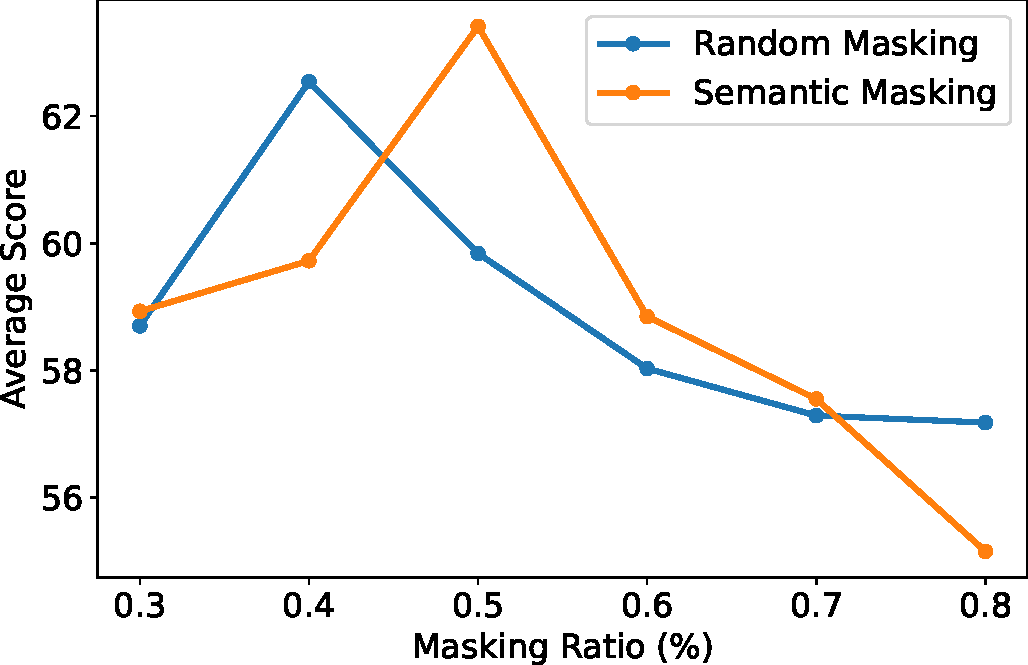
\includegraphics[width=.45 \textwidth]{figures/acc_vs_mask_ratio_cos_rnd.pdf}
    \caption{\textbf{Masking ratio}. The y-axes are LVU average accuracy scores. A moderate masking ratio of $40-50\%$ works well for attentive probing.}
    \label{fig:cos_mask_ablation}
    \vspace{-1.0em}
\end{figure}

\begin{table}[]
\centering
\caption{\textbf{Encoder depth}. A deep encoder can improve accuracy. Here, we use attentive probing and Top 1 accuracy. We evaluated on LVU (Avg.), Breakfast (BF), and COIN datasets. Default settings are marked in \colorbox{baselinecolor}{gray}.}
\vspace{-1.5em}
\begin{center}
\label{tab:encoder_depth}
\tablestyle{10pt}{1.05}
\begin{tabular}{cccc}
\hline

\hline

\hline
\textbf{Depth} & \textbf{LVU} & \textbf{BF} & \textbf{COIN} \\
\hline
16 & 59.73 & 87.04 & 92.47 \\
24 & 60.04 & 89.58 & \textbf{93.26} \\
32 & \baseline{\textbf{63.41}} & \baseline{\textbf{90.70}} & \baseline{91.8} \\
\hline

\hline

\hline
\end{tabular}
\end{center}
\vspace{-2.0em}
\end{table}



\begin{figure*}[ht]
    \centering
    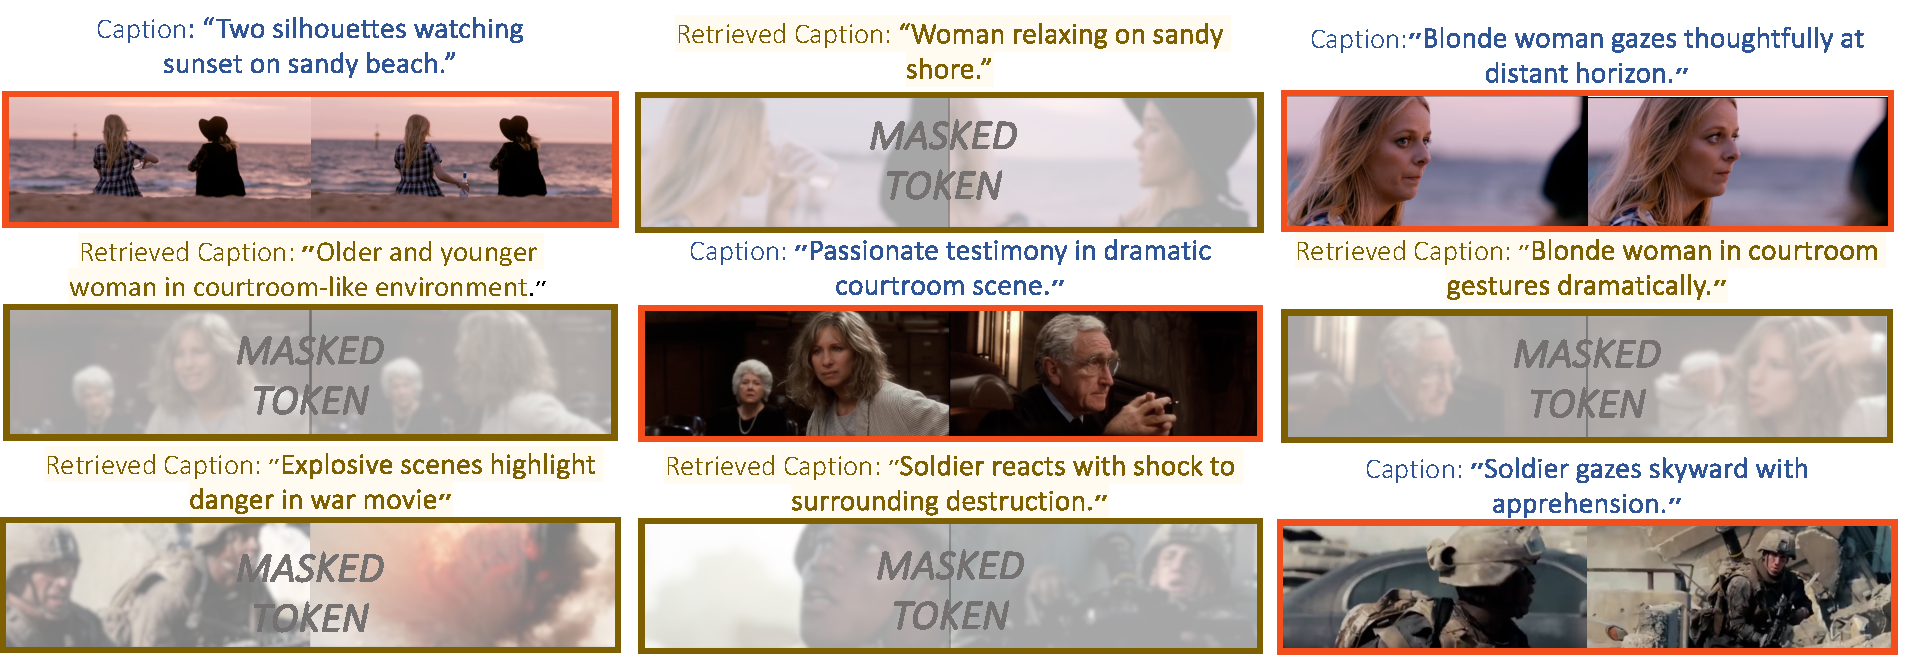
\includegraphics[width=1.\textwidth]{figures/interp_results.pdf} 
    \caption{\textbf{Interpretable predictions -- examples}: Each row visualizes three consecutive five-second segments. Above each segment, we show the original caption for the visible tokens and the retrieved caption for the reconstructed masked tokens. As shown, the model successfully reconstructs the semantic meaning of the masked embeddings, offering insight into the model's effectiveness and capabilities.}
    \label{fig:interp_res}
\end{figure*}

\begin{figure}[ht]
    % \centering
    \hspace{1cm}
    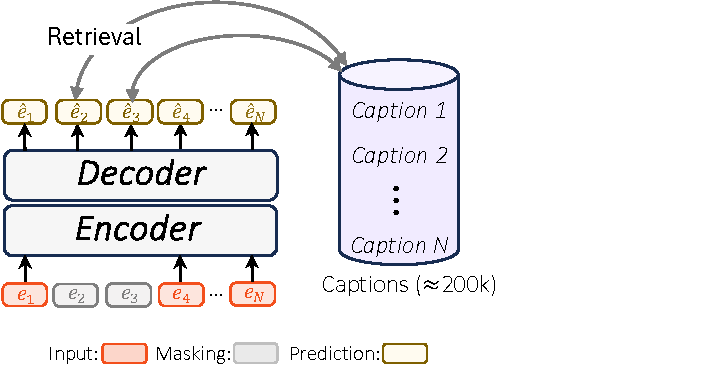
\includegraphics[width=.5\textwidth]{figures/interpretation_scheme.pdf}
    \caption{\textbf{Interpretable predictions -- scheme}: For each reconstructed masked embedding, we perform retrieval against a large set of captions collected from the MovieClip dataset. The top matches can then be used to assess the model's quality.}
    \label{fig:interp_scheme}
\vspace{-2.0em}
\end{figure}

\subsection{Interpretable Predictions Experiment}
\label{sec:exp_interpretabitlity}
The ability to understand model predictions is essential to facilitate human understanding of what the model learns. In Sec.~\ref{subsec:interpretability} we propose an interpretability technique for our framework. In this section, we show its effectiveness and verify the reconstructions produced by the decoder. 
In practice, we used the MovieClips dataset to extract captions. For each short-video segment, $v_i$, in the dataset, we generate concise annotations, $a_i$, using the Claude Sonnet 3.5 LLM \cite{anthropic2024claude35sonnet}. Next, we sample a long video from the dataset and extract its corresponding embeddings, $\mathcal{E}$, masking $40\%$ of them. Our model is fed with the visible embeddings and tasked with reconstructing all embeddings, resulting in the predicted set, $\hat{\mathcal{E}}$. Each annotation is transformed into a language embedding using LanguageBind, which has the same embedding space as $\mathcal{E}$. Using the cosine similarity, we perform retrieval by selecting the most similar textual embeddings. We conduct this retrieval for both the original embeddings, $\mathcal{E}$, and the predicted embeddings, $\hat{\mathcal{E}}$. We provide a scheme of the process in Figure~\ref{fig:interp_scheme}. The original model retrieval accuracy (R@5) is 75.34\%.

For concise visualization of the results, in Fig.~\ref{fig:interp_res}, we subsample short video segments and present the interpreted model's predictions. We observe that in most cases, our model predicts embeddings that are semantically close to the original ones. This means that the predicted embeddings align with either the same or semantically similar enough textual embedding. As expected, we observe that the retrieved textual embeddings tend to be more abstract or high-level, rather than precise descriptions of the scene. For instance, in one example, the ground truth annotation is ``Blonde woman sips drink by the sea'', while the retrieved annotation according to the prediction is "Woman relaxing on sandy shore." This behavior is akin to what has been observed with MAE models in the image domain~\cite{he2022masked}, where predicted image patches are often blurry and lack fine details. Similarly, our model’s predictions can be seen as abstract representations, capturing the essence of a scene but missing some specific details. 
